\documentclass[xcolor=dvipsnames,10pt]{beamer}

\mode<presentation>

\usepackage{beamerthemesplit}
\usepackage[italian]{babel}
\usepackage[utf8]{inputenc}
\usepackage{multirow}

\graphicspath{ {./images/} }

\usecolortheme[named=MidnightBlue]{structure}

%Warsaw Dresden Singapore Copenhagen Madrid AnnArbor
\usetheme{Warsaw}
\setbeamercovered{transparent}
\setbeamercolor{lowercolor}{fg=white , bg=MidnightBlue}
\setbeamertemplate{blocks}[rounded][shadow=true]
\setbeamertemplate{items}[default]
\setbeamertemplate{navigation symbols}{}

\def\hilite<#1>{%
\temporal<#1>{\color{lightgray}}{\color{black}}%
{\color{black}}}

\usetitlepagetemplate{
  \begin{center}
    %\pgfuseimage{salom}
    %\vskip0.5ex
    \textsc{Università degli Studi di Firenze}
    \vskip1ex
    \scriptsize{\textsc{Dipartimento di Sistemi e Informatica} }\\
    \scriptsize{\textsc{Tesi di Laurea Triennale in Ingegneria Informatica } }
    \vskip4ex
    \begin{beamerboxesrounded}[lower=lowercolor, shadow=true]{}
     \begin{center}
    \normalsize{Analisi e sviluppo di una web application \\
		basata sui framework JPA, JSF, CDI, \\
		per l'amministrazione di attività di trasferimento tecnologico\\}
     \end{center}
    \end{beamerboxesrounded}

    \vskip4ex
    \begin{footnotesize}
\begin{columns}[t]
\begin{column}{0.2\textwidth}
\begin{flushright}
\vskip -3em
      \begin{minipage}[t]{20ex}
	\raggedright
	\emph{Candidati:}\\
	Tommaso Levato\\ Alessio Sarullo\\ Giulio Galvan
      \end{minipage}
\end{flushright}
\end{column}
\begin{column}{0.4\textwidth}
\vskip-3ex
  \begin{figure}
   
\includegraphics[width=2.5cm]{images/stemma.pdf}
  \end{figure}
\end{column}
\begin{column}{0.3\textwidth}
	\emph{Relatori}\\
	Prof. Enrico Vicario\\
 \vskip 0.5em
	\emph{Correlatori}\\
	Ing. Jacopo Torrini\\
\end{column}
\end{columns}
      \vskip 4ex
      \rule{15em}{0.4pt}
      \vskip 0.2ex
      Anno Accademico 2012/2013
\vskip 0.3em
\begin{itemize}
\item \structure{Obiettivo}: \\Sviluppo di una applicazione web per la gestione delle convenzioni
\end{itemize}
    \end{footnotesize}
  \end{center}
}

\title[Analisi e sviluppo di una web application]{Analisi e sviluppo di una web application \\
basata sui framework JPA, JSF, CDI, \\
per l'amministrazione di attività di trasferimento tecnologico\\}
\author{Tommaso Levato, Alessio Sarullo, Giulio Galvan}

\date{\today}

\newcommand*\oldmacro{}%
\let\oldmacro\insertshorttitle%
\renewcommand*\insertshorttitle{%
  \oldmacro\hfill%
  \insertframenumber\,/\,\inserttotalframenumber}

\begin{document}

\frame{\titlepage}
\section{Introduzione}
\subsection{Contesto Applicativo}
\begin{frame}{Convenzione}
\vskip2ex
... un accordo fra l'Università, rappresentata da un docente, ed una azienda, per la realizzazione di un prodotto.
\vskip2ex

le fasi :\\
\vskip2ex
  \begin{enumerate}
    \item Il docente si accorda con un'azienda riguardo ad un progetto.
    \item Il docente, insieme al RAS, valuta i costi e stila la Tabella di Ripartizione dei compensi.
    \item Il RAS prepara un documento da discutere nel prossimo Consiglio di Dipartimento, che deciderà se approvare o meno la convenzione.
    \item In caso di approvazione la convenzione viene \textbf{inserita nell'applicazione}.
    \item ...
    \item La convenzione risulta esaurita (l'importo stabilito è stato pagato interamente) .
  \end{enumerate}
\end{frame}

\begin{frame}{Gestione di una Convenzione}
 \vskip-3ex
 L'applicazione deve \textbf{monitorare} la convenzione dal suo inserimento fino a quando risulti esaurita. 
 \vskip5ex
 In questo intervallo di tempo l'applicazione deve consentire di \textbf{compiere delle operazioni} sulla convenzione.
\end{frame}

\subsection{Requisiti}
\begin{frame}{Requisiti principali}
  \vskip-3ex
  L'applicazione deve consentire di:\\
  \vskip3ex
  \begin{itemize}
   \item inserire convenzioni
   \item inserire rate per una convenzione
   \item visualizzare le convenzioni inserite
   \item aggiornare i dati di una convenzione
   \item notificare le scadenze
  \end{itemize}

\end{frame}

\section{Analisi}
  \begin{frame}{Agenti}
    \vskip-3ex
    \begin{itemize}
     \item L'Operatore:\\
     \vskip3ex
      \begin{itemize}
       \item inserisce, modifica convenzioni
       \item inserisce le rate
      \end{itemize}
     \vskip3ex
     \item Il Docente:\\
      \begin{itemize}
       \item visualizza lo stato delle proprie convenzioni
      \end{itemize}
     \vskip3ex
     \item Il Tempo:\\
      \begin{itemize}
       \item notifica le scadenze
      \end{itemize}

    \end{itemize}

    
  \end{frame}

  \subsection{Casi d'Uso}
  \begin{frame}{Casi d'uso dell'Operatore}
    \begin{figure}[h]
    \label{use_case_diag_operator}
    \centering
    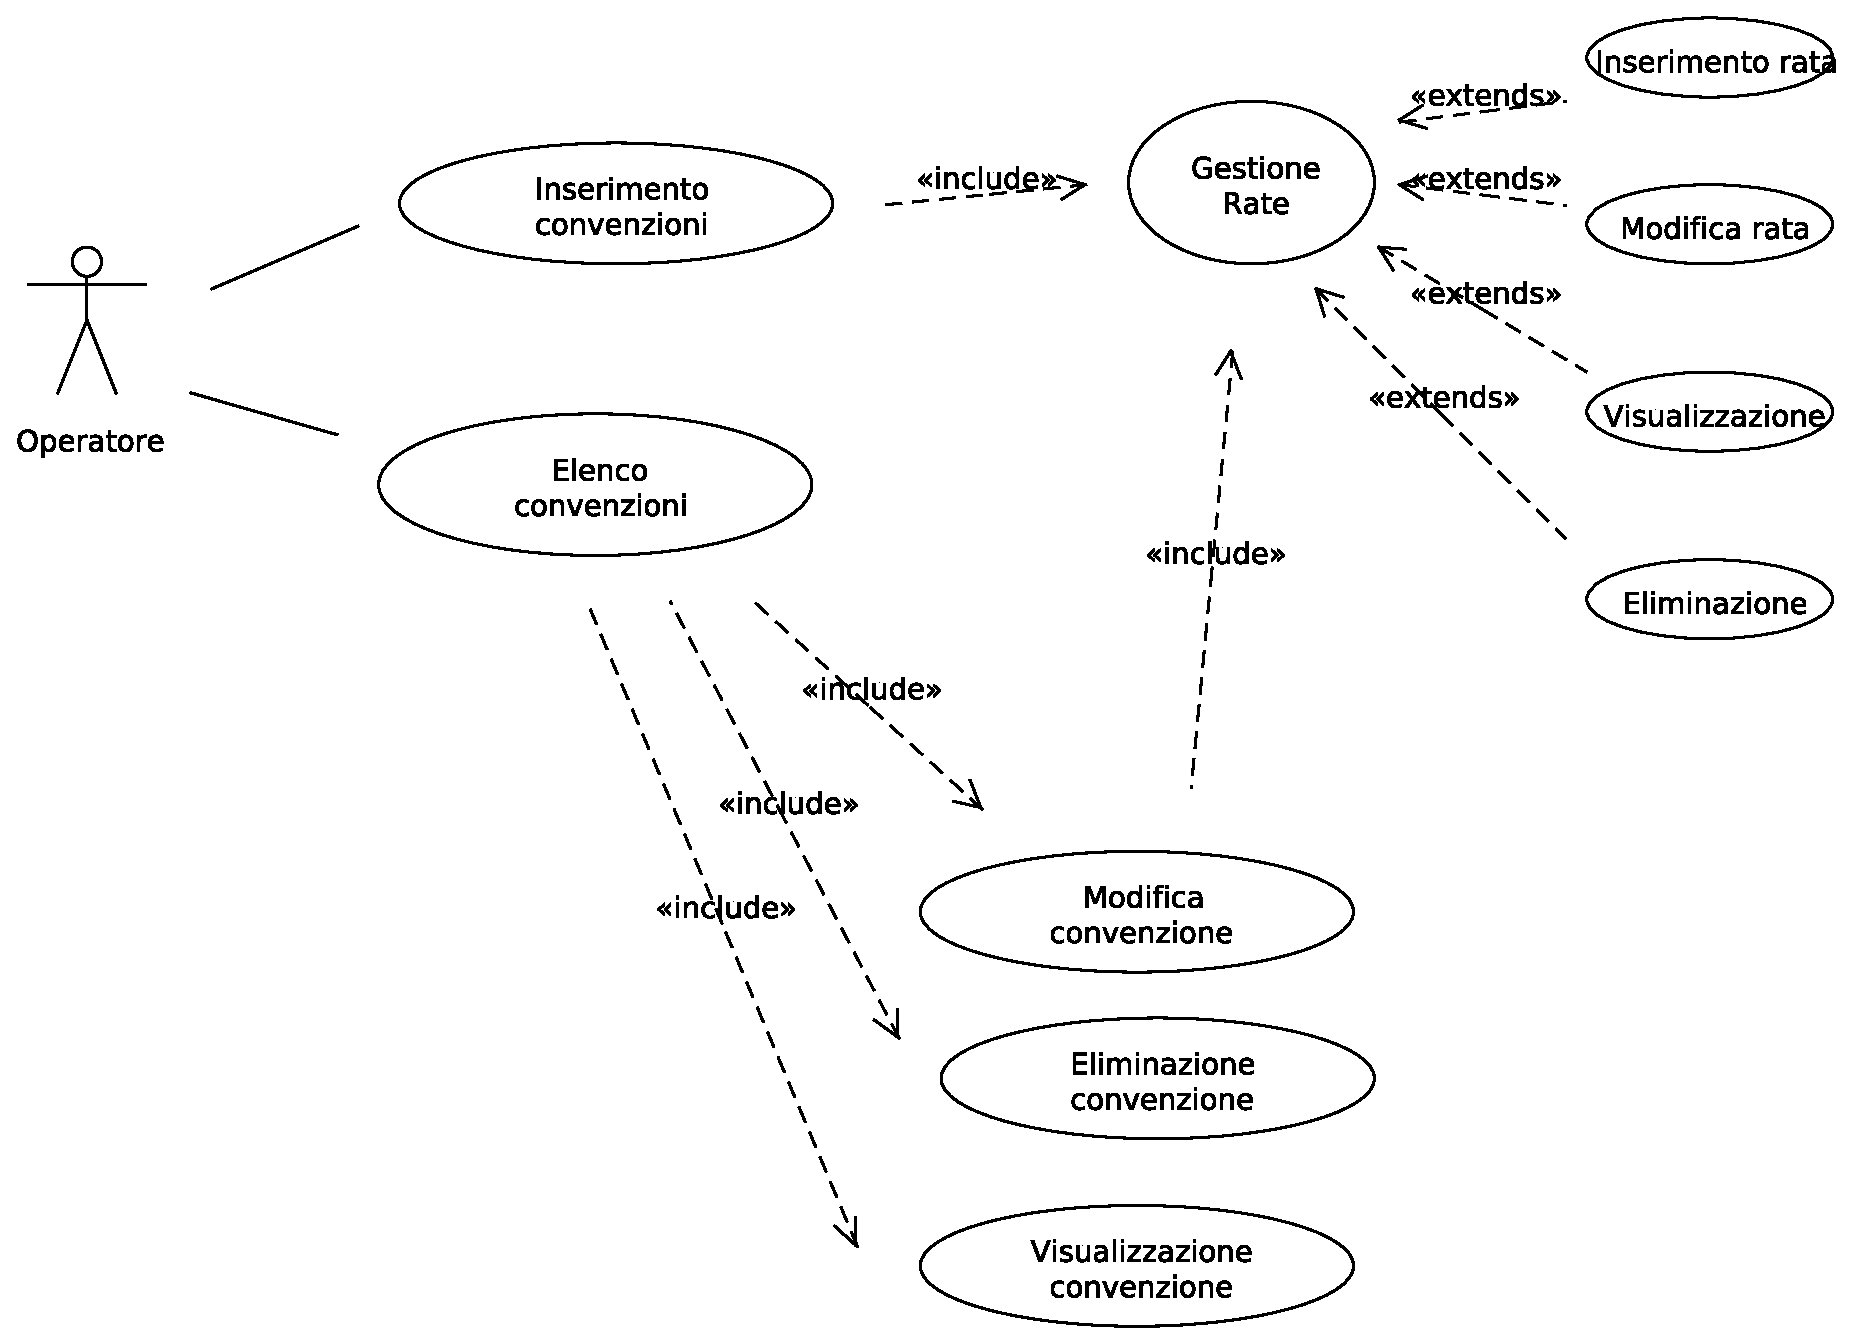
\includegraphics[height=0.8\textheight, width=0.7\textwidth]{images/casi_uso_operatore_semplified.eps}
    \end{figure}
  \end{frame}
  
  \begin{frame}{Esempio di caso d'uso}
   
   \vskip-2ex
      \begin{beamerboxesrounded}[lower=lowercolor, shadow=true]{}
     \begin{center}
	\normalsize{Inserimento di una nuova convenzione\\}
     \end{center}
    \end{beamerboxesrounded}
  
  \vskip2ex
  \textbf{Percorso base}:
  l'Operatore, una volta effettuato il login, clicca su ``Crea una convenzione"; viene visualizzata una schermata suddivisa in varie schede,
  ognuna corrispondente ad un passo della procedura. I passi sono:
  \begin{enumerate}
    \item Inserimento dei dati della convenzione\\
      \begin{itemize}
	\item Il titolo
	\item L'importo totale
	\item ...
      \end{itemize}
            
    \item Inserimento della tabella di ripartizione\\
    \item Inserimento delle rate  
    \item Inserimento della documentazione relativa alla convenzione\\
    \vskip2ex
    
    L'Operatore clicca su ``Salva," la convenzione viene salvata e la procedura termina. Si ritorna alla schermata precedente.
    
  \end{enumerate}
  \end{frame}
  
  \begin{frame}{Esempio di caso d'uso}
  

  \textbf{Percorso alternativo 1}:
  l'Operatore clicca sul tasto ``Salva'' o ``Successivo'' senza aver compilato alcuni dei campi obbligatori, o avendo inserito dei valori non consentiti; viene visualizzato un messaggio di errore 
  e il documento non viene salvato. La schermata non viene cambiata, dando la possibilità all'Operatore di procedere alla correzione.

  
  \vskip3ex
  
  \textbf{Percorso alternativo 2}:
  durante uno qualsiasi dei passi, l'Operatore  clicca sul tasto ``Annulla'', che comporta, a seguito di una conferma, il ritorno alla schermata precedente
  senza che la convenzione venga inserita o i cambiamenti effettuati salvati.
  

   
   
  \end{frame}
  
  \begin{frame}{}
     \begin{figure}[h]
      \centering
      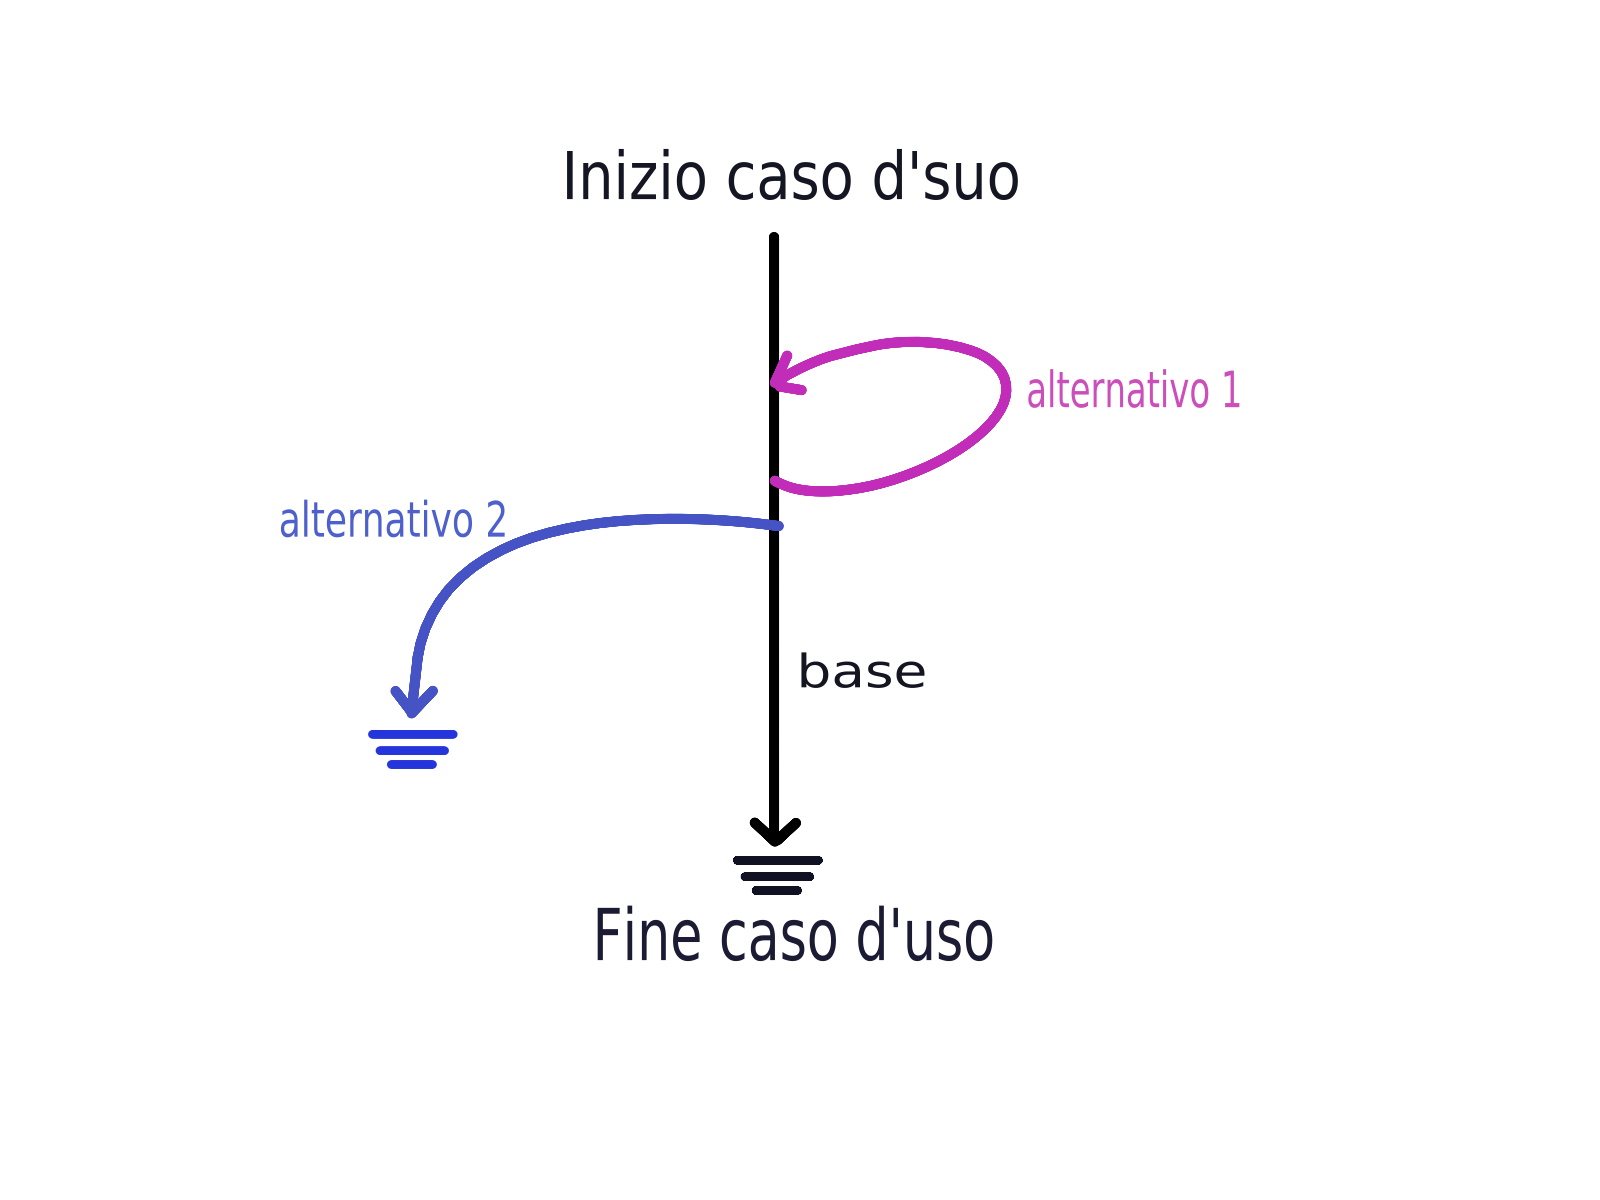
\includegraphics[scale=0.25]{images/flows.png}
    \end{figure}
   
  \end{frame}


  
  \begin{frame}{Casi d'uso del Docente}
    \begin{figure}[h]
      \label{use_case_diag_teacher}
      \centering
      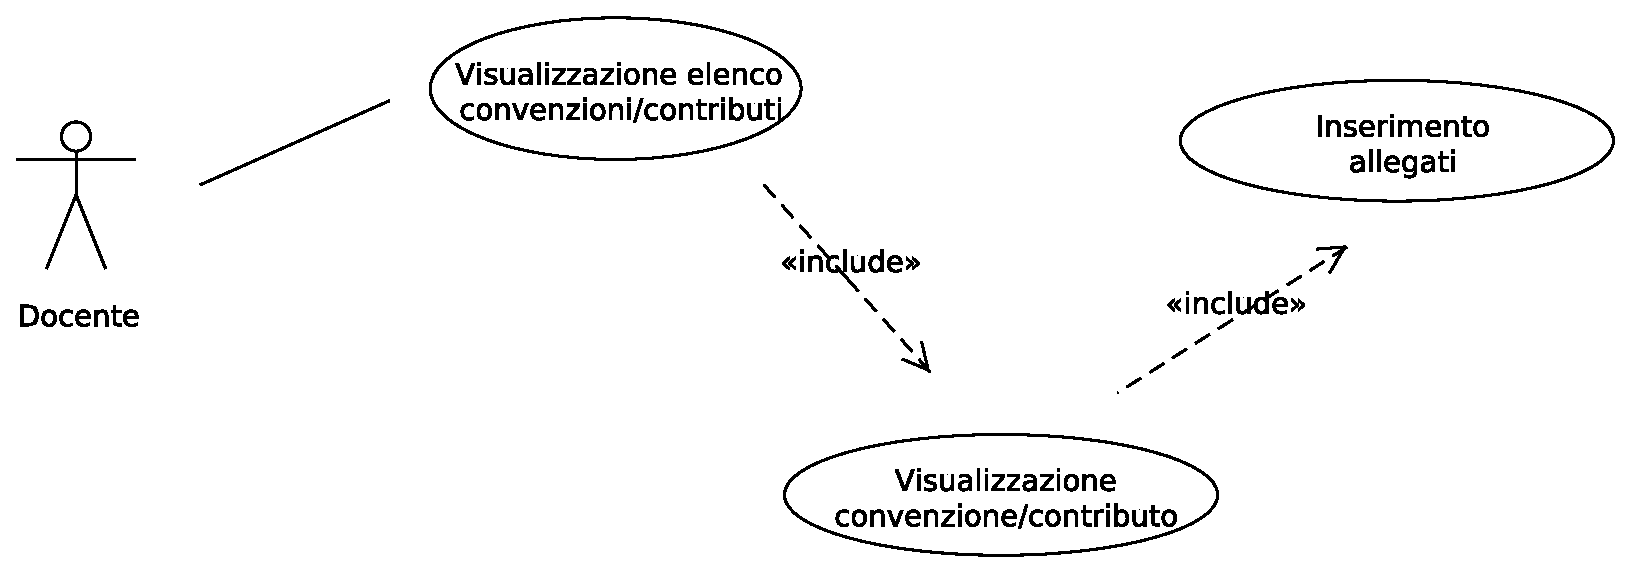
\includegraphics[width=0.8\textwidth]{images/casi_uso_docente.eps}
    \end{figure}
  \end{frame}
  
  \begin{frame}{Casi d'uso del Tempo}
    \begin{figure}[h]
      \label{use_case_diag_time}
      \centering
      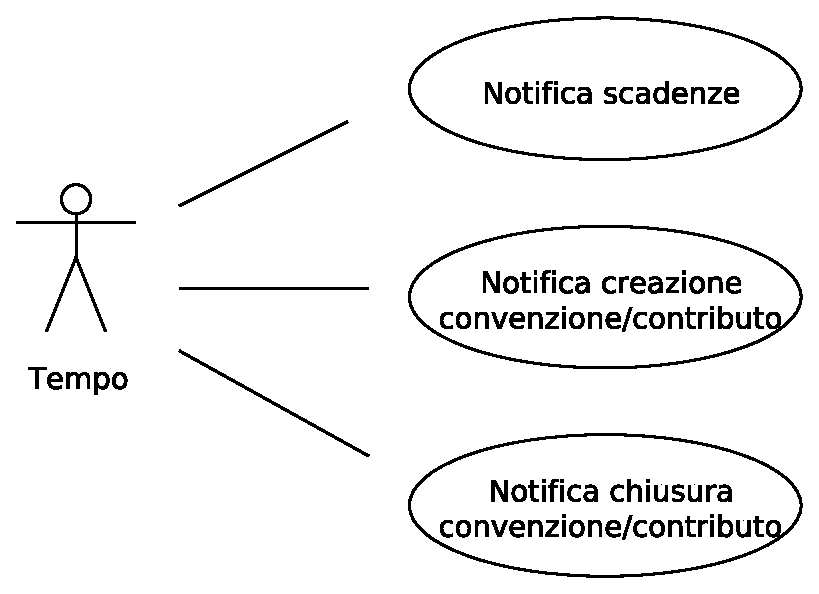
\includegraphics[width = 0.5\textwidth]{images/casi_uso_tempo.eps}
    \end{figure}
  \end{frame}


  
  \subsection{Modello di Business}
  \begin{frame}{Gli oggetti del modello}
     \begin{itemize}
      \item Convenzione
      \item Rata
      \item Responsabile Scientifico
      \item Ditta
      \item ...
     \end{itemize}

   
  \end{frame}
  
  \begin{frame}{Diagramma delle classi}
  
    \begin{figure}[h]
      \label{business_model}
      \centering
      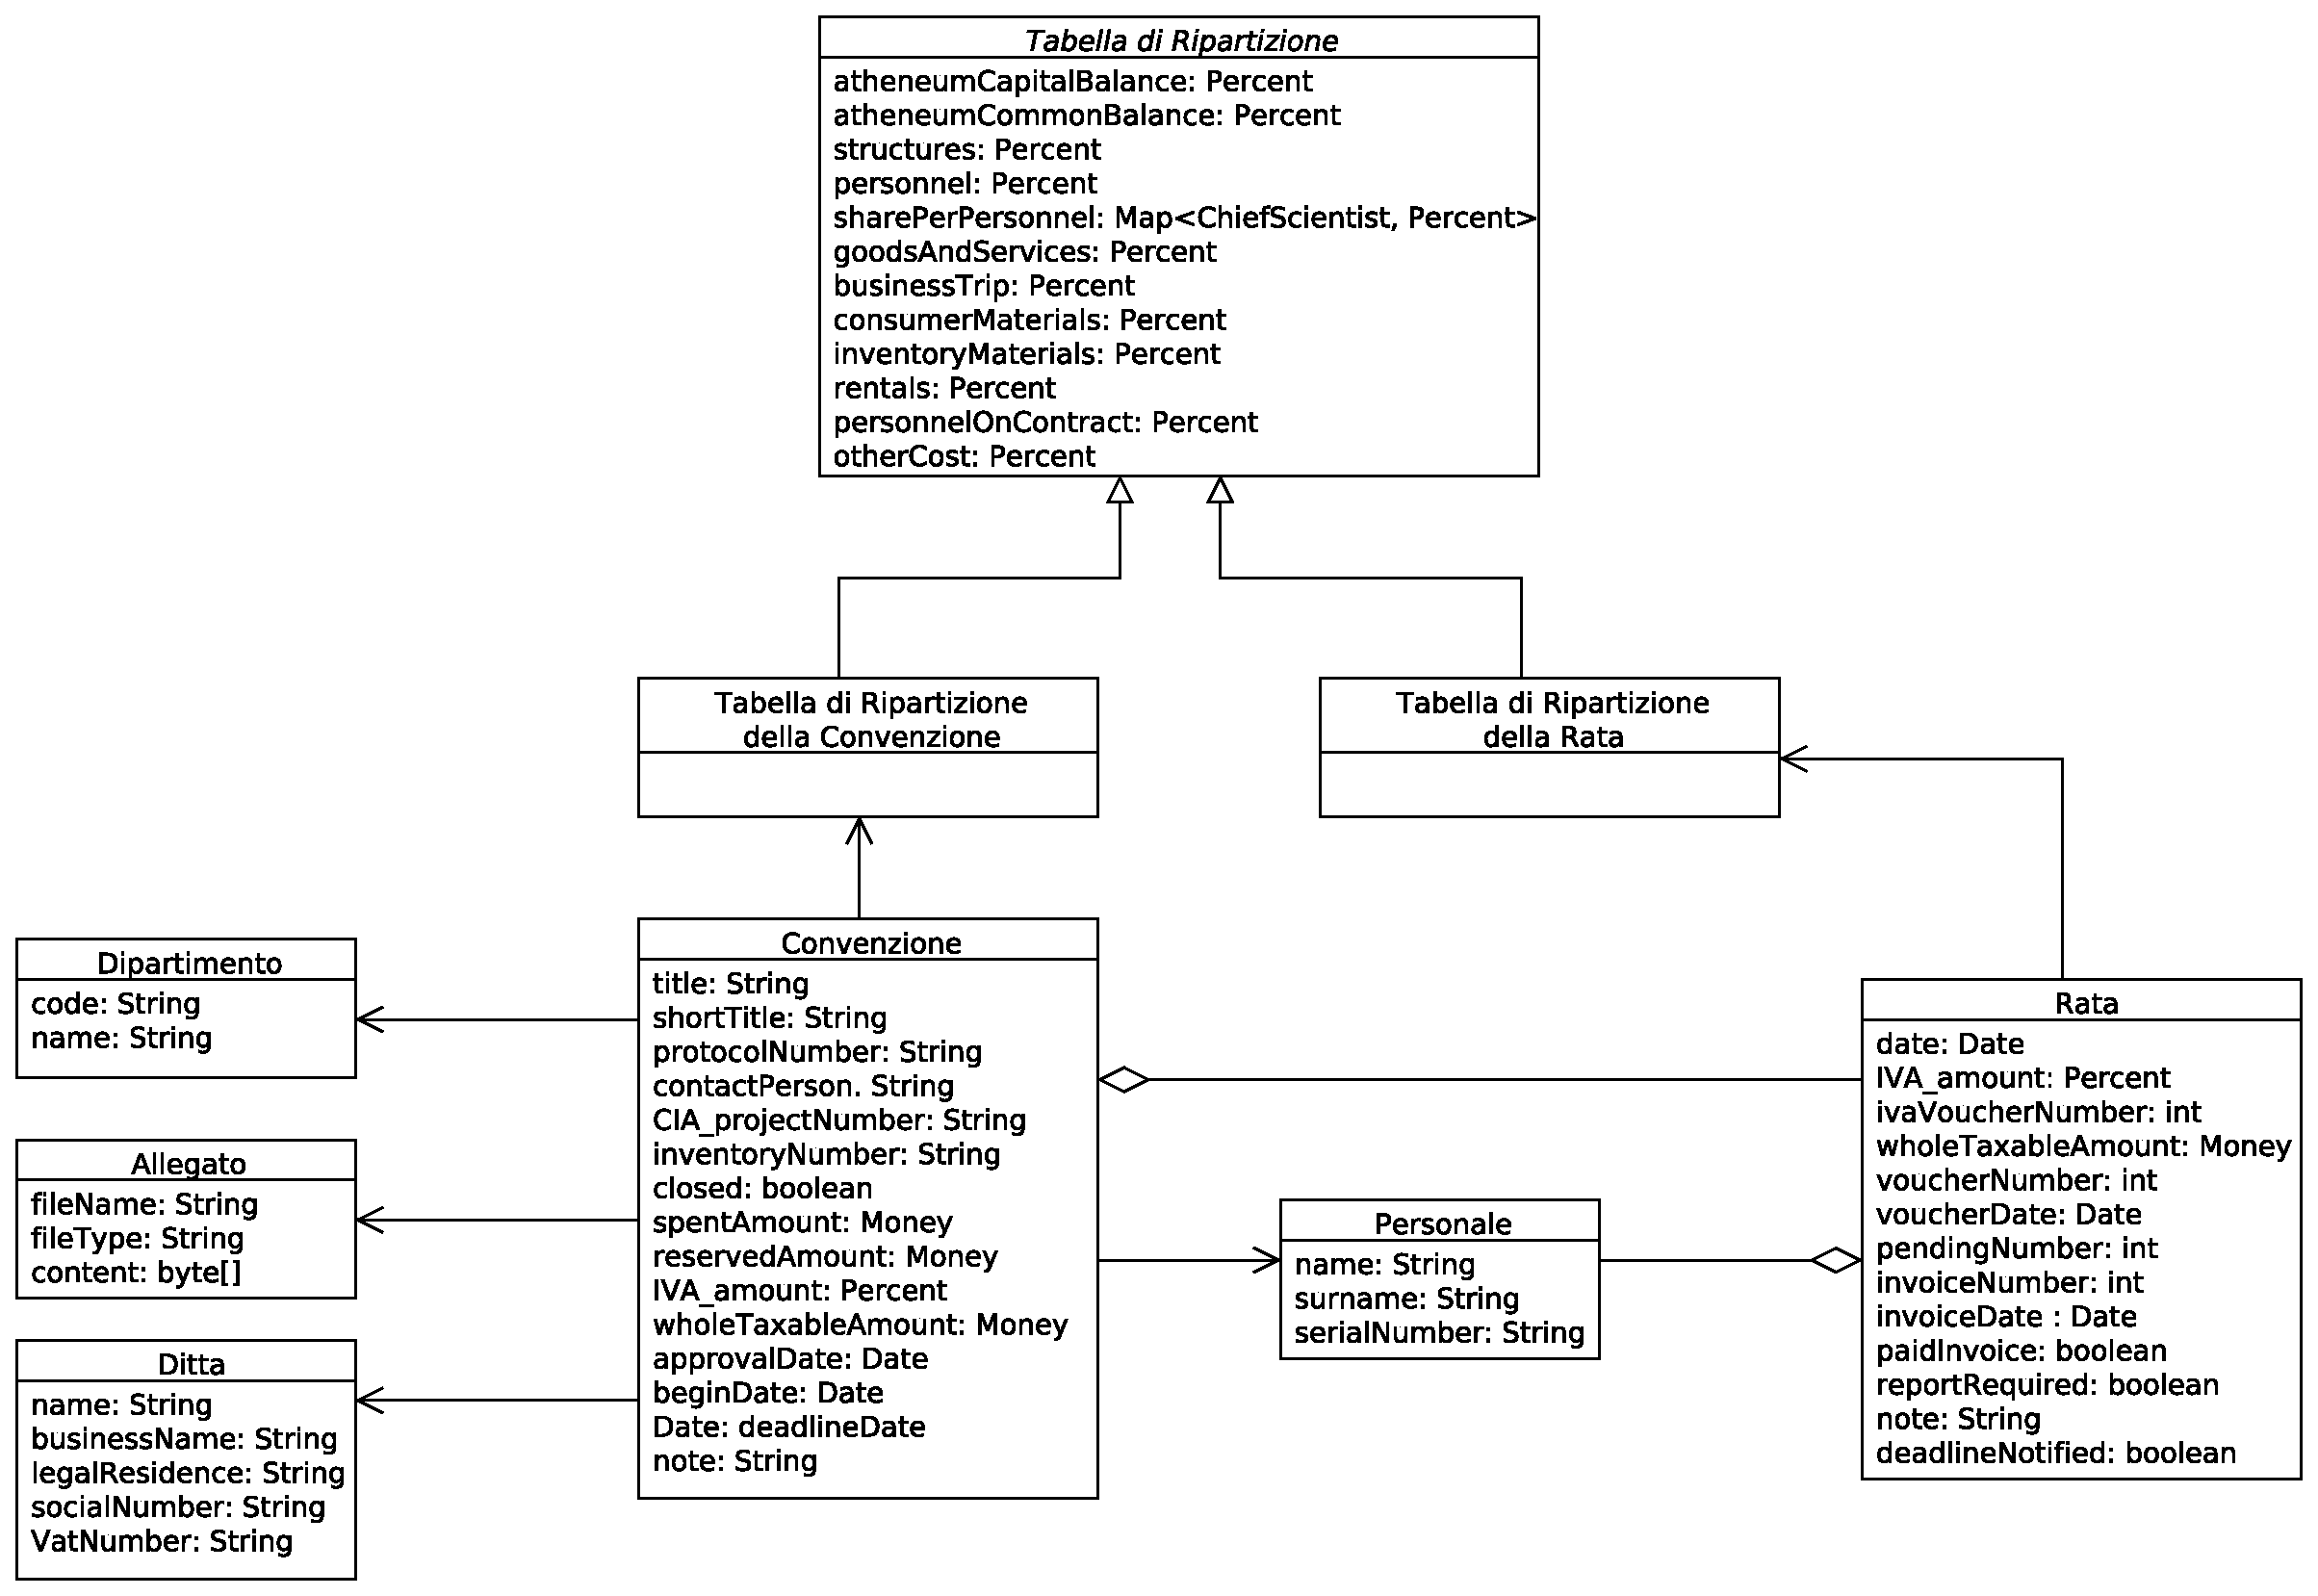
\includegraphics[width=0.8\textwidth]{images/modello_business_simplified.eps}
    \end{figure}
   
  \end{frame}


  
  




\section{Tecnologie}

\subsection{Introduzione}

\begin{frame}{Tecnologie utilizzate}

\begin{itemize}
\item JBoss AS 7.1
	\begin{itemize}
	\item fornisce l'infrastruttura per consentire l'esecuzione di una web application
	\end{itemize}

\item Java EE 6
	\begin{itemize}
	\item piattaforma software per lo sviluppo di applicazioni enterprise
	\item comprende varie tecnologie, fra cui:
		\begin{itemize}
		\item JPA (Java Persistence API) 2.0
		\item CDI (Contexts and Dependency Injection) 1.0
		\item JSF (JavaServer Faces) 2.0
		\end{itemize}
		
	\end{itemize}

\end{itemize}


\end{frame}

\begin{frame}{Bean}

\begin{itemize}
\item Sono componenti software riusabili che possono essere gestiti dal container

\item Vari tipi:
	\begin{itemize}
	
	\item \textsl{Enterprise JavaBeans} (EJB): bean utilizzati per la logica di business o la persistenza
		\begin{itemize}
		\item session bean
		\item message-driven bean
		\item entity bean
		\end{itemize}
		
	\item  \textsl{Managed beans}: bean utilizzati a livello di presentazione
	\end{itemize}

\end{itemize}

\end{frame}


\subsection{JPA}
\begin{frame}{Java Persistence API}

\begin{itemize}
\item Si occupa della persistenza dei dati
\end{itemize}

\begin{itemize}
\item Problema:

	\begin{itemize}
	\item Nelle applicazioni enterprise è necessario ricorrere ad un database
	
	\item Il modello più utilizzato all'interno dei database è il \textsl{modello relazionale}
		\begin{itemize}
		\item le entità sono le \textsl{relazioni}
		\item sono collegate tra di loro mediante \textsl{chiavi}
		\end{itemize}
	
	\item Il modello utilizzato all'interno delle applicazioni Java è il \textsl{modello a oggetti}
		\begin{itemize}
		\item le entità sono le \textsl{classi}
		\item sono collegate tra di loro mediante \textsl{riferimenti}
		\end{itemize}
	
	\end{itemize}

\end{itemize}

\end{frame}


\begin{frame}{Integrazione fra i modelli}

\begin{itemize}
\item Occorre un sistema per la conversione tra i due modelli

	\begin{itemize}
	\item non deve influire pesantemente sullo sviluppo dell'applicazione
	\item in particolare, deve garantire:
	
		\begin{itemize}
		\item trasparenza rispetto al modello di dominio
		\item recupero di informazioni indipendente dal database
		\item compatibilità con database preesistenti
		\end{itemize}
	
	\end{itemize}

\end{itemize}

\end{frame}


\begin{frame}{Costrutti fondamentali}

\begin{itemize}
\item Entità
	\begin{itemize}
	\item è un'unità che possiede uno stato e può essere persistita
	\item una classe Java è un'entità se:
		\begin{itemize}
		\item è annotata \texttt{@Entity}
		\item ha un costruttore senza parametri
		\end{itemize}
	\end{itemize}

\item Entity Manager
	\begin{itemize}
	\item gestisce le entità
	\item è associato ad un \textsl{Persistence Context}
		\begin{itemize}
		\item è l'insieme delle entità gestite da un Entity Manager in un dato momento
		\item se un entità fa parte di un Persistence Context viene detta \textsl{managed}
		\item altrimenti viene detta \textsl{detached}
		\end{itemize}
	\end{itemize}

\end{itemize}	


\end{frame}

\begin{frame}{Query}

\begin{itemize}
\item Si usa il \textsl{Java Persistence Query Language} (JPQL)

\item Sintassi simile a SQL, ma:

	\begin{itemize}
	\item è indipendente dal database
	\item utilizza le entità del modello di dominio e relativi attributi
	\end{itemize}


\end{itemize}

\end{frame}


\subsection{CDI}

\begin{frame}{Contexts and Dependency Injection}

\begin{itemize}
\item Problema: incompatibilità tra
	\begin{itemize}
	\item il livello di business, che usa EJB;
	\item il livello di presentazione, che usa Managed bean.
	\end{itemize}
	
\item CDI:
	\begin{itemize}
	\item consente l'utilizzo di EJB nel livello di presentazione
	\item fornisce una specifica per la definizione di Managed bean
	\end{itemize}
\end{itemize}

\end{frame}



\begin{frame}{Panoramica}

\begin{itemize}
\item Servizi offerti:
	\begin{itemize}
	\item Contesto
	\item Iniezione di dipendenza
	\end{itemize}

\item Caratteristiche principali:
	\begin{itemize}
	\item integrazione Expression Language
	\item disaccoppiamento
	\item controllo sui tipi
	\end{itemize}
\end{itemize}

\end{frame}

\begin{frame}{Bean CDI}

\begin{itemize}
\item \textsl{Scope}
	\begin{itemize}
	\item lega il bean ad un particolare contesto
	\item determina il ciclo di vita
	\item limita la visibilità al client
	\end{itemize}
	
\item 4 possibili scope:
	\begin{itemize}
	\item Request
	\item Conversation
	\item Session
	\item Application
	\end{itemize}

\end{itemize}

\end{frame}



\subsection{JSF}

\begin{frame}{JavaServer Faces}

\begin{itemize}
\item Framework per lo sviluppo di interfaccia grafica
\item \textsl{Component-based}
\item Consente estensione delle funzionalità tramite librerie di terze parti
\end{itemize}

\end{frame}


\begin{frame}{Architettura}

\begin{itemize}
\item Architettura Model-View-Controller
\end{itemize}

\begin{figure}
	\centering
	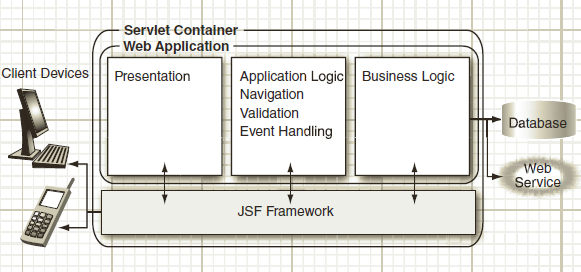
\includegraphics[width=0.5\textwidth]{JSF_architecture.png}
\end{figure}

\end{frame}


\begin{frame}{Comunicazione client-server}
\begin{figure}
	\centering
	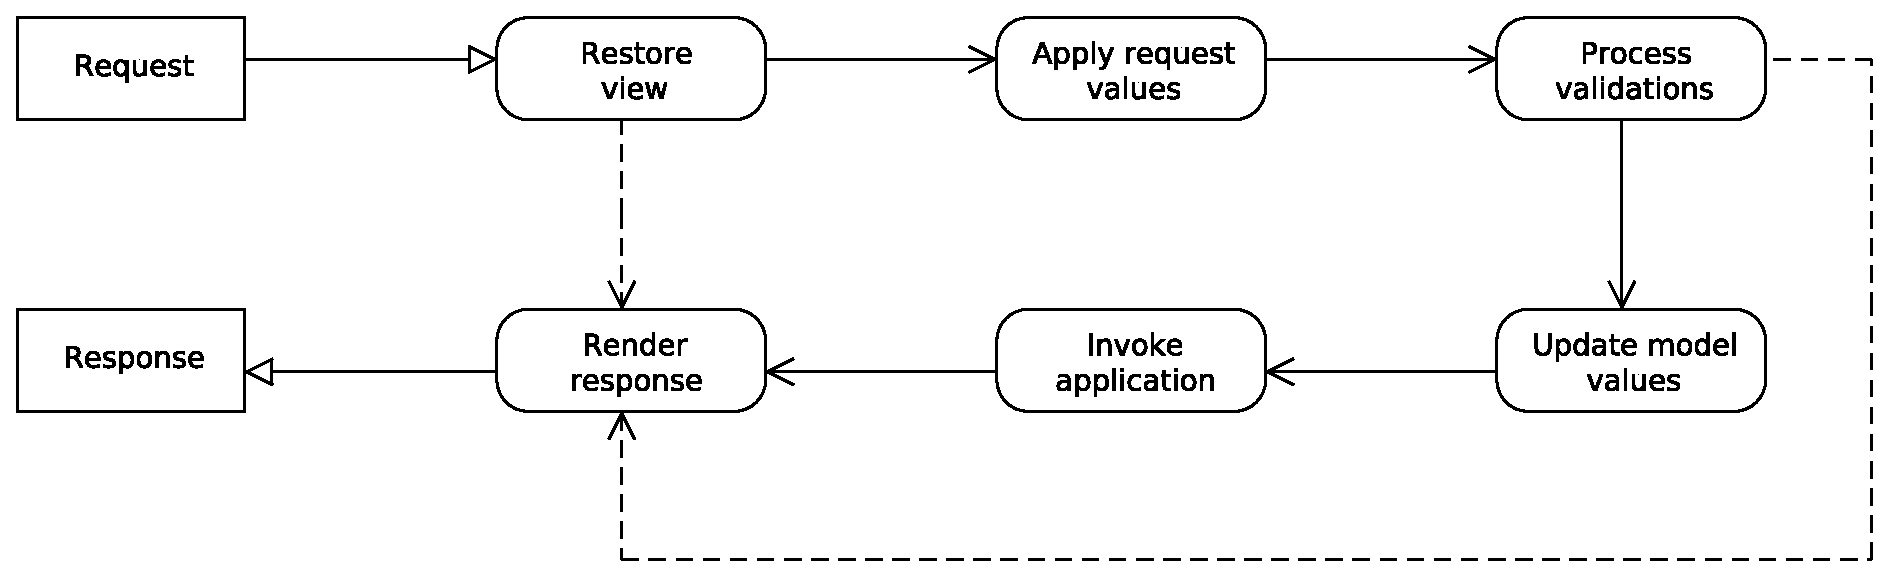
\includegraphics[width=1\textwidth]{custom_JSF_lifecycle.eps}
\end{figure}

\end{frame}

























\subsection{Deltaspike}

\begin{frame}[fragile]{Deltaspike}


\begin{itemize}
\item Framework che estende le funzionalità di CDI
\vspace{0.8em}
\item \textsl{Annotation-based}

\begin{lstlisting}[basicstyle={\tiny\ttfamily}]
&&@Secures&&
&&@AlterCompaniesAllowed&&
public boolean canUserAlterCompanies() {...}
\end{lstlisting}

\item Gestisce i permessi degli utenti
\end{itemize}


\end{frame}

\begin{frame}[fragile]{Architettura}
\begin{columns}[T]
\begin{column}{.5\textwidth}


\begin{itemize}
\item Sicurezza su base metodo

	\begin{itemize}
	\item Classe \textsl{Authorizer}
	\vspace{0.8em}
	\item Annotare i metodi\newline
	da controllare
	\end{itemize}

\vspace{0.8em}
\item Sicurezza su base pagina
	\begin{itemize}
	\item Gerarchia interfacce/classi -\textgreater  cartelle/pagine
	\vspace{0.8em}
	\item Interfaccia \textsl{AccessDecisionVoter}
	\vspace{0.8em}
	\item Possibilità di specificare\newline
	una pagina di errore\newline
	con un messaggio adatto
	\end{itemize}
\end{itemize}
\end{column}

\begin{column}{.5\textwidth}
\vspace{2.6em}
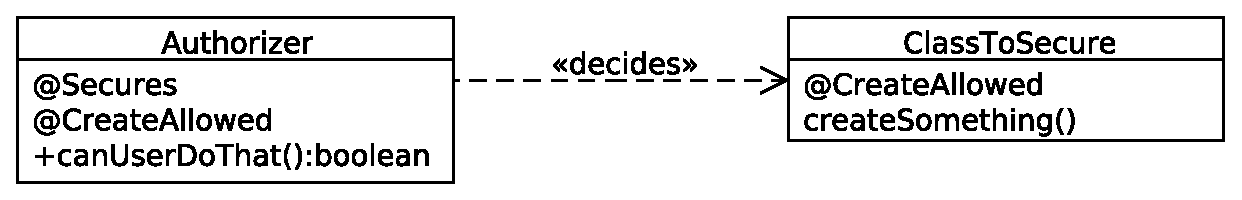
\includegraphics[width=1\textwidth]{deltaspikeMethod.eps}

\vspace{1.6em}
\begin{lstlisting}[basicstyle={\tiny\ttfamily}]

interface Pages{
    &&@Secured&&(value = { MyVoter.class }, 
    errorView = MyErrorPage.class)
    class AgreementWiz implements ViewConfig {
    }

    &&@Secured&&(value = { MyOtherVoter.class },
    errorView = MyOtherErrorPage.class)
    class Home implements ViewConfig {
    }
    
    class MyErrorPage {}
    class MyOtherErrorPage{}
}
\end{lstlisting}

\end{column}

\end{columns}
\end{frame}

\begin{frame}{Pagina di errore}
\centering
	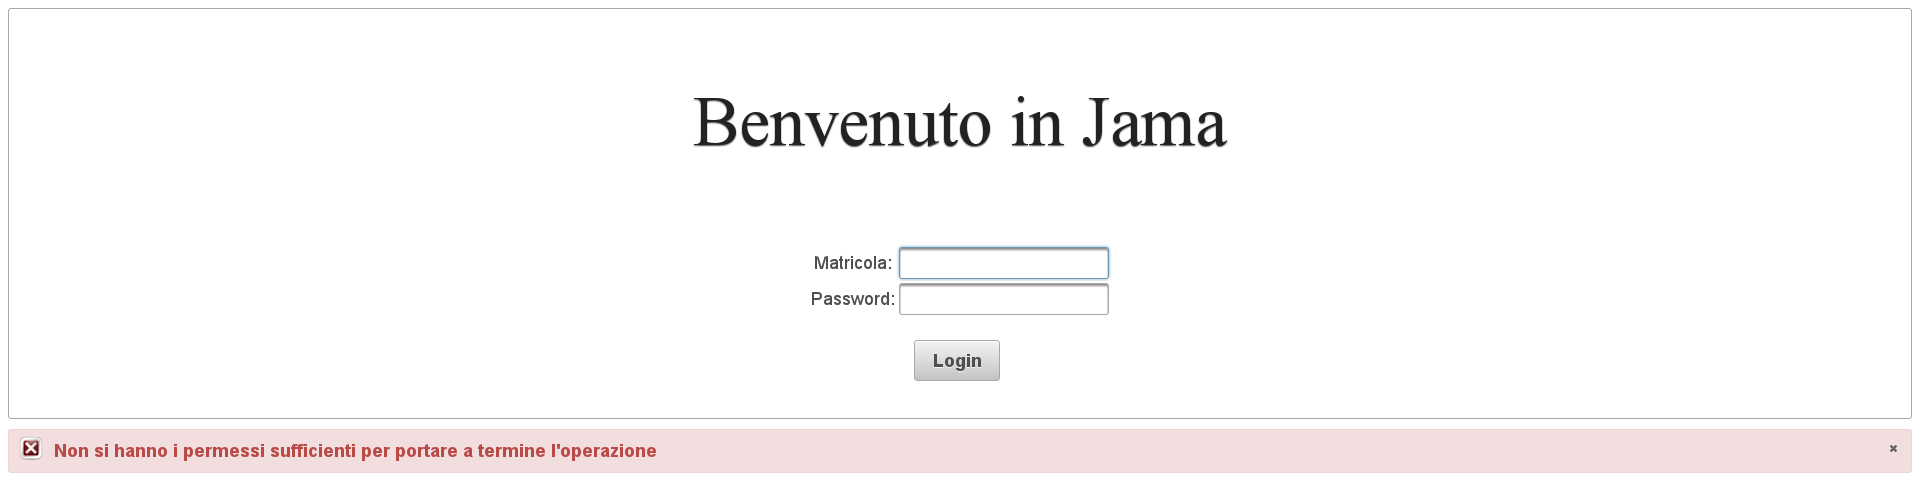
\includegraphics[width=1\textwidth]{PermessiInsufficienti.png}
\end{frame}

\subsection{LDAP}
\begin{frame}{Lightweight Directory Access Protocol}
\begin{columns}[T]
\begin{column}{.5\textwidth}
\begin{itemize}
\item Protocollo per accesso a cartelle
\item Utilizzato da Jama per recupero utenti
\item Libreria JLDAP
\end{itemize}
\end{column}

\begin{column}{.5\textwidth}
\vspace{0.7em}
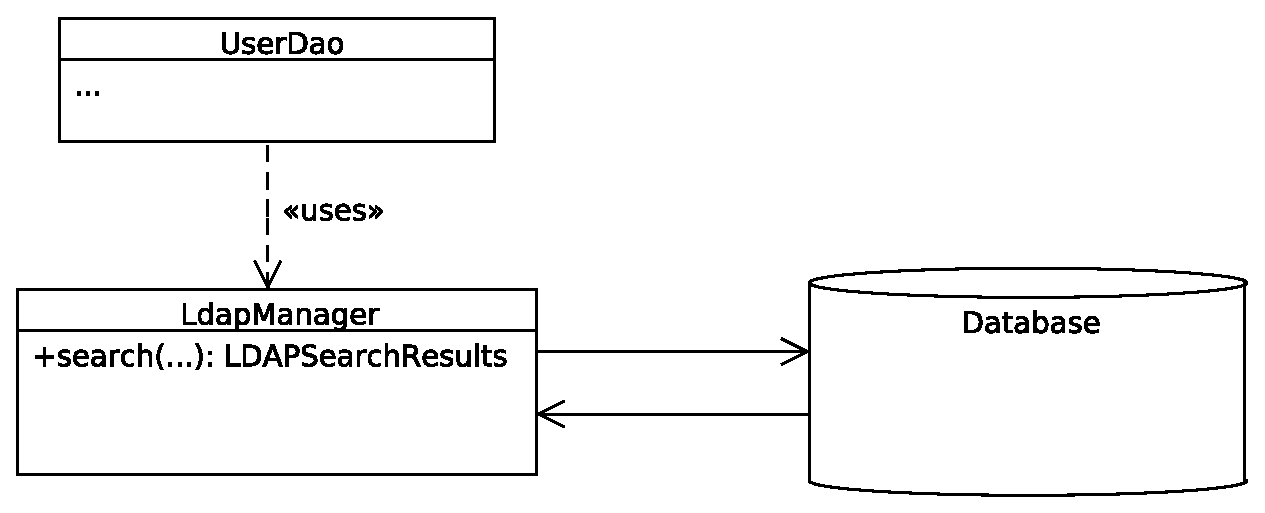
\includegraphics[width=1\textwidth]{Ldap.eps}
\end{column}




\end{columns}

\end{frame}


\section{Utenti}
\subsection{Modello}
\begin{frame}{Modello degli Utenti}
\begin{itemize}
\item Descrive la struttura delle classi riguardanti gli utenti\newline
ed i loro permessi
\end{itemize}	

\vspace{0.8em}
\centering
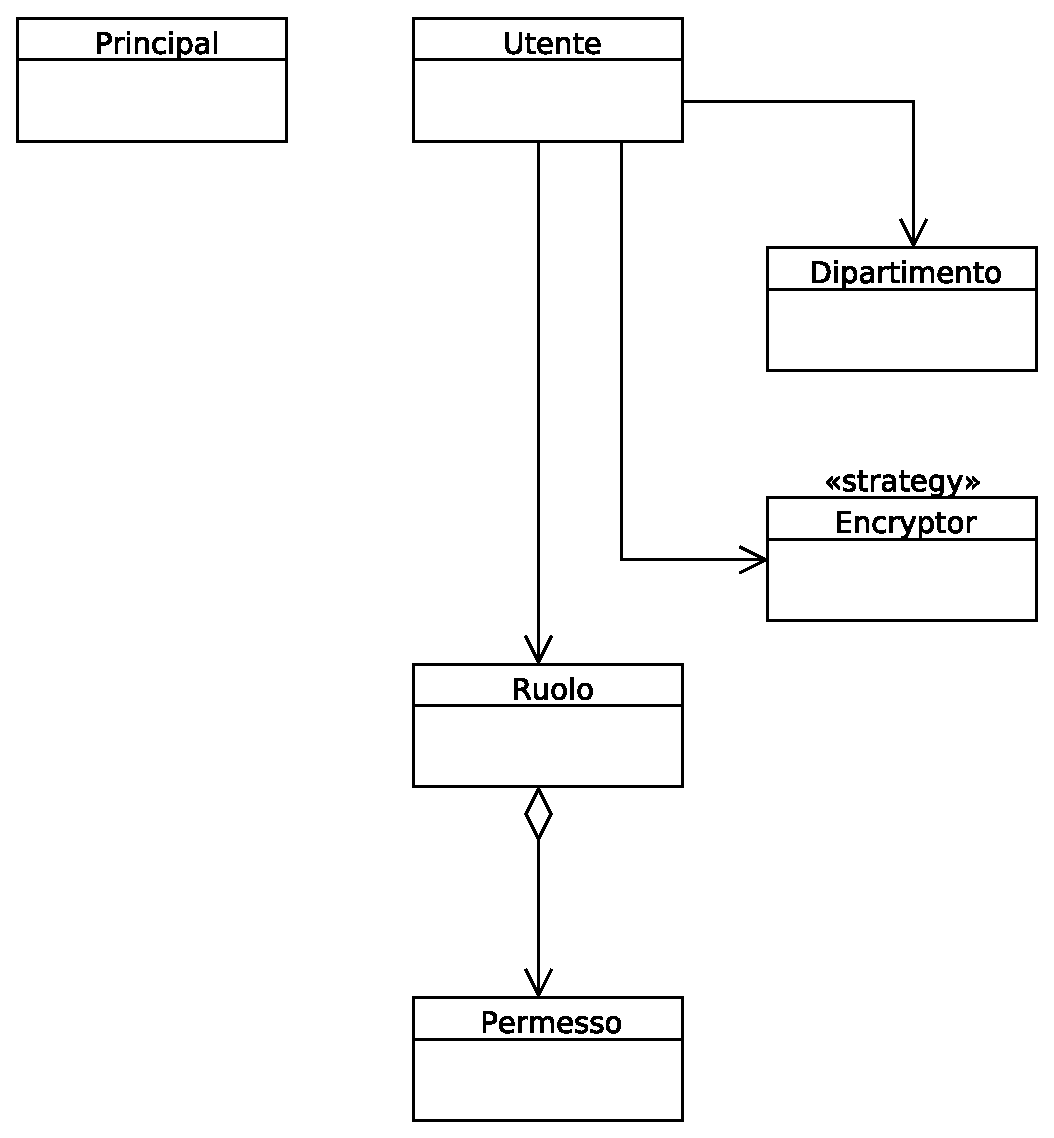
\includegraphics[width=0.4\textwidth]{user_model_final.eps}

\end{frame}

\subsection{Ruoli e Permessi}

\begin{frame}{Ruoli e Permessi}
\begin{itemize}
	
\item Operatore Amministrativo
	\begin{itemize}
	\item Gestisce le convenzioni del proprio dipartimento
	\end{itemize}

\vspace{0.8em}
\item Docente
	\begin{itemize}
	\item Visualizza le proprie convenzioni
	\item Allega documenti alle proprio convenzioni
	\end{itemize}

\vspace{0.8em}
\item Ospite
	\begin{itemize}
	\item Nessun permesso
	\end{itemize}

\vspace{0.8em}
\item Amministratore
	\begin{itemize}
	\item Gestisce gli utenti ed i loro permessi
	\item Non afferisce a nessun dipartimento
	\end{itemize}
\end{itemize}
\end{frame}

\section{Collaudo}
\subsection{Introduzione}
\begin{frame}{Collaudo}
\begin{itemize}
\item Verifica le funzionalità dell'applicazione
\vspace{0.8em}
\item Suddivisione in scenari con ragionevole copertura\newline
dei casi d'uso
\end{itemize}

\end{frame}

\begin{frame}{Scenari e Casi di test}

\begin{itemize}
\item Copertura dei casi d'uso
\end{itemize}

\begin{center}
\footnotesize
\begin{tabular}{| c| p{4.5cm} | p{4.5cm} |} 
    \hline
     & Descrizione & Casi di test esercitati \\
    \hline
    1 & Inserimento convenzione,\newline
    aggiunta ditta,
    aggiunta rata & UC \#OA1 base,
    UC \#OA10 alt3,\newline
    UC \#OA6 base\\
    \hline
    2 & Modifica rata contributo & UC \#OA2 base,
    UC \#OA3 base, \newline
    UC \#OA7 base  \\
    \hline
    3 & Modifica dati ditta & UC \#OA13 base,
    UC \#OA11 base \\
    \hline
    4 & Inserimento contributo con allegati & UC \#OA1 base\\
    \hline
    5 & Inserimento allegato convenzione & UC \#D1 base,
    UC \#D3 base\\
    \hline
    6 & Aggiunta utente & UC \#A1 base\\
    \hline
  \end{tabular} 
\end{center}

\end{frame}

\subsection{Risultati}

\begin{frame}{Risultati}
\begin{center}
\footnotesize
\begin{tabular}{|c|p{2.5cm}|p{3cm}|p{1.5cm}|c|}
    \hline
    Passo & Descrizione sequenza operazioni & Risultato
     atteso & Risultato\newline ottenuto & Ok\\
    \hline
    1 & L'Amministratore clicca sul pulsante\newline ``Aggiungi utente'' & Viene visualizzata una schermata contenente\newline i campi da inserire& Uguale 
      al\newline risultato\newline atteso& Sì\\
    \hline
    2 & L'Amministratore riempie i campi quindi clicca su ``Salva''& Si torna alla\newline pagina iniziale & Uguale al\newline risultato\newline atteso & Sì \\
    \hline
     3 & L'Amministratore clicca su ``Visualizza lista utenti''& Compare una lista contenente tutti gli utenti, fra i quali anche quello appena inserito & Uguale al\newline risultato\newline atteso & Sì \\
    \hline
\end{tabular}
\end{center}

\end{frame}

\section{Conclusioni}
\begin{frame}{Riassunto}
\begin{itemize}
\item Copertura del ciclo di sviluppo di un'applicazione
	\vspace{0.6em}
	\begin{itemize}
	\item requisiti acquisiti da un'audience informata
	\vspace{0.4em}
	\item applicazione progettata, sviluppata, collaudata e\newline
	pronta per andare in produzione (DINFO, DIEF, DICEA)
	\end{itemize}
\vspace{1em}
\item Ulteriori sviluppi abilitati
\vspace{0.6em}
\begin{itemize}
\item gestione dei contratti
\vspace{0.4em}
\item autorizzazioni ad incarichi retribuiti
\end{itemize}
\end{itemize}

\end{frame}
\begin{frame}{Requisiti}
\begin{itemize}
\item Gestione delle convenzioni e dei contributi
\vspace{0.8em}
	\begin{itemize}
	\item inserire convenzioni
	\item inserire rate per una convenzione
	\item visualizzare convenzioni inserite
	\item aggiornare i dati di una convenzione
	\item notificare le scadenze
	\end{itemize}
\end{itemize}
\end{frame}

\begin{frame}{Conclusioni}
\begin{columns}[T]
\begin{column}{.3\textwidth}
\begin{itemize}
\item Tecnologie
\vspace{0.8em}
	\begin{itemize}
	\item JPA
	\vspace{0.6em}
	\item CDI
	\vspace{0.6em}
	\item JSF
	\vspace{0.6em}
	\item Deltaspike
	\vspace{0.6em}
	\item LDAP
\end{itemize}
\end{itemize}
\end{column}

\begin{column}{.55\textwidth}

\centering
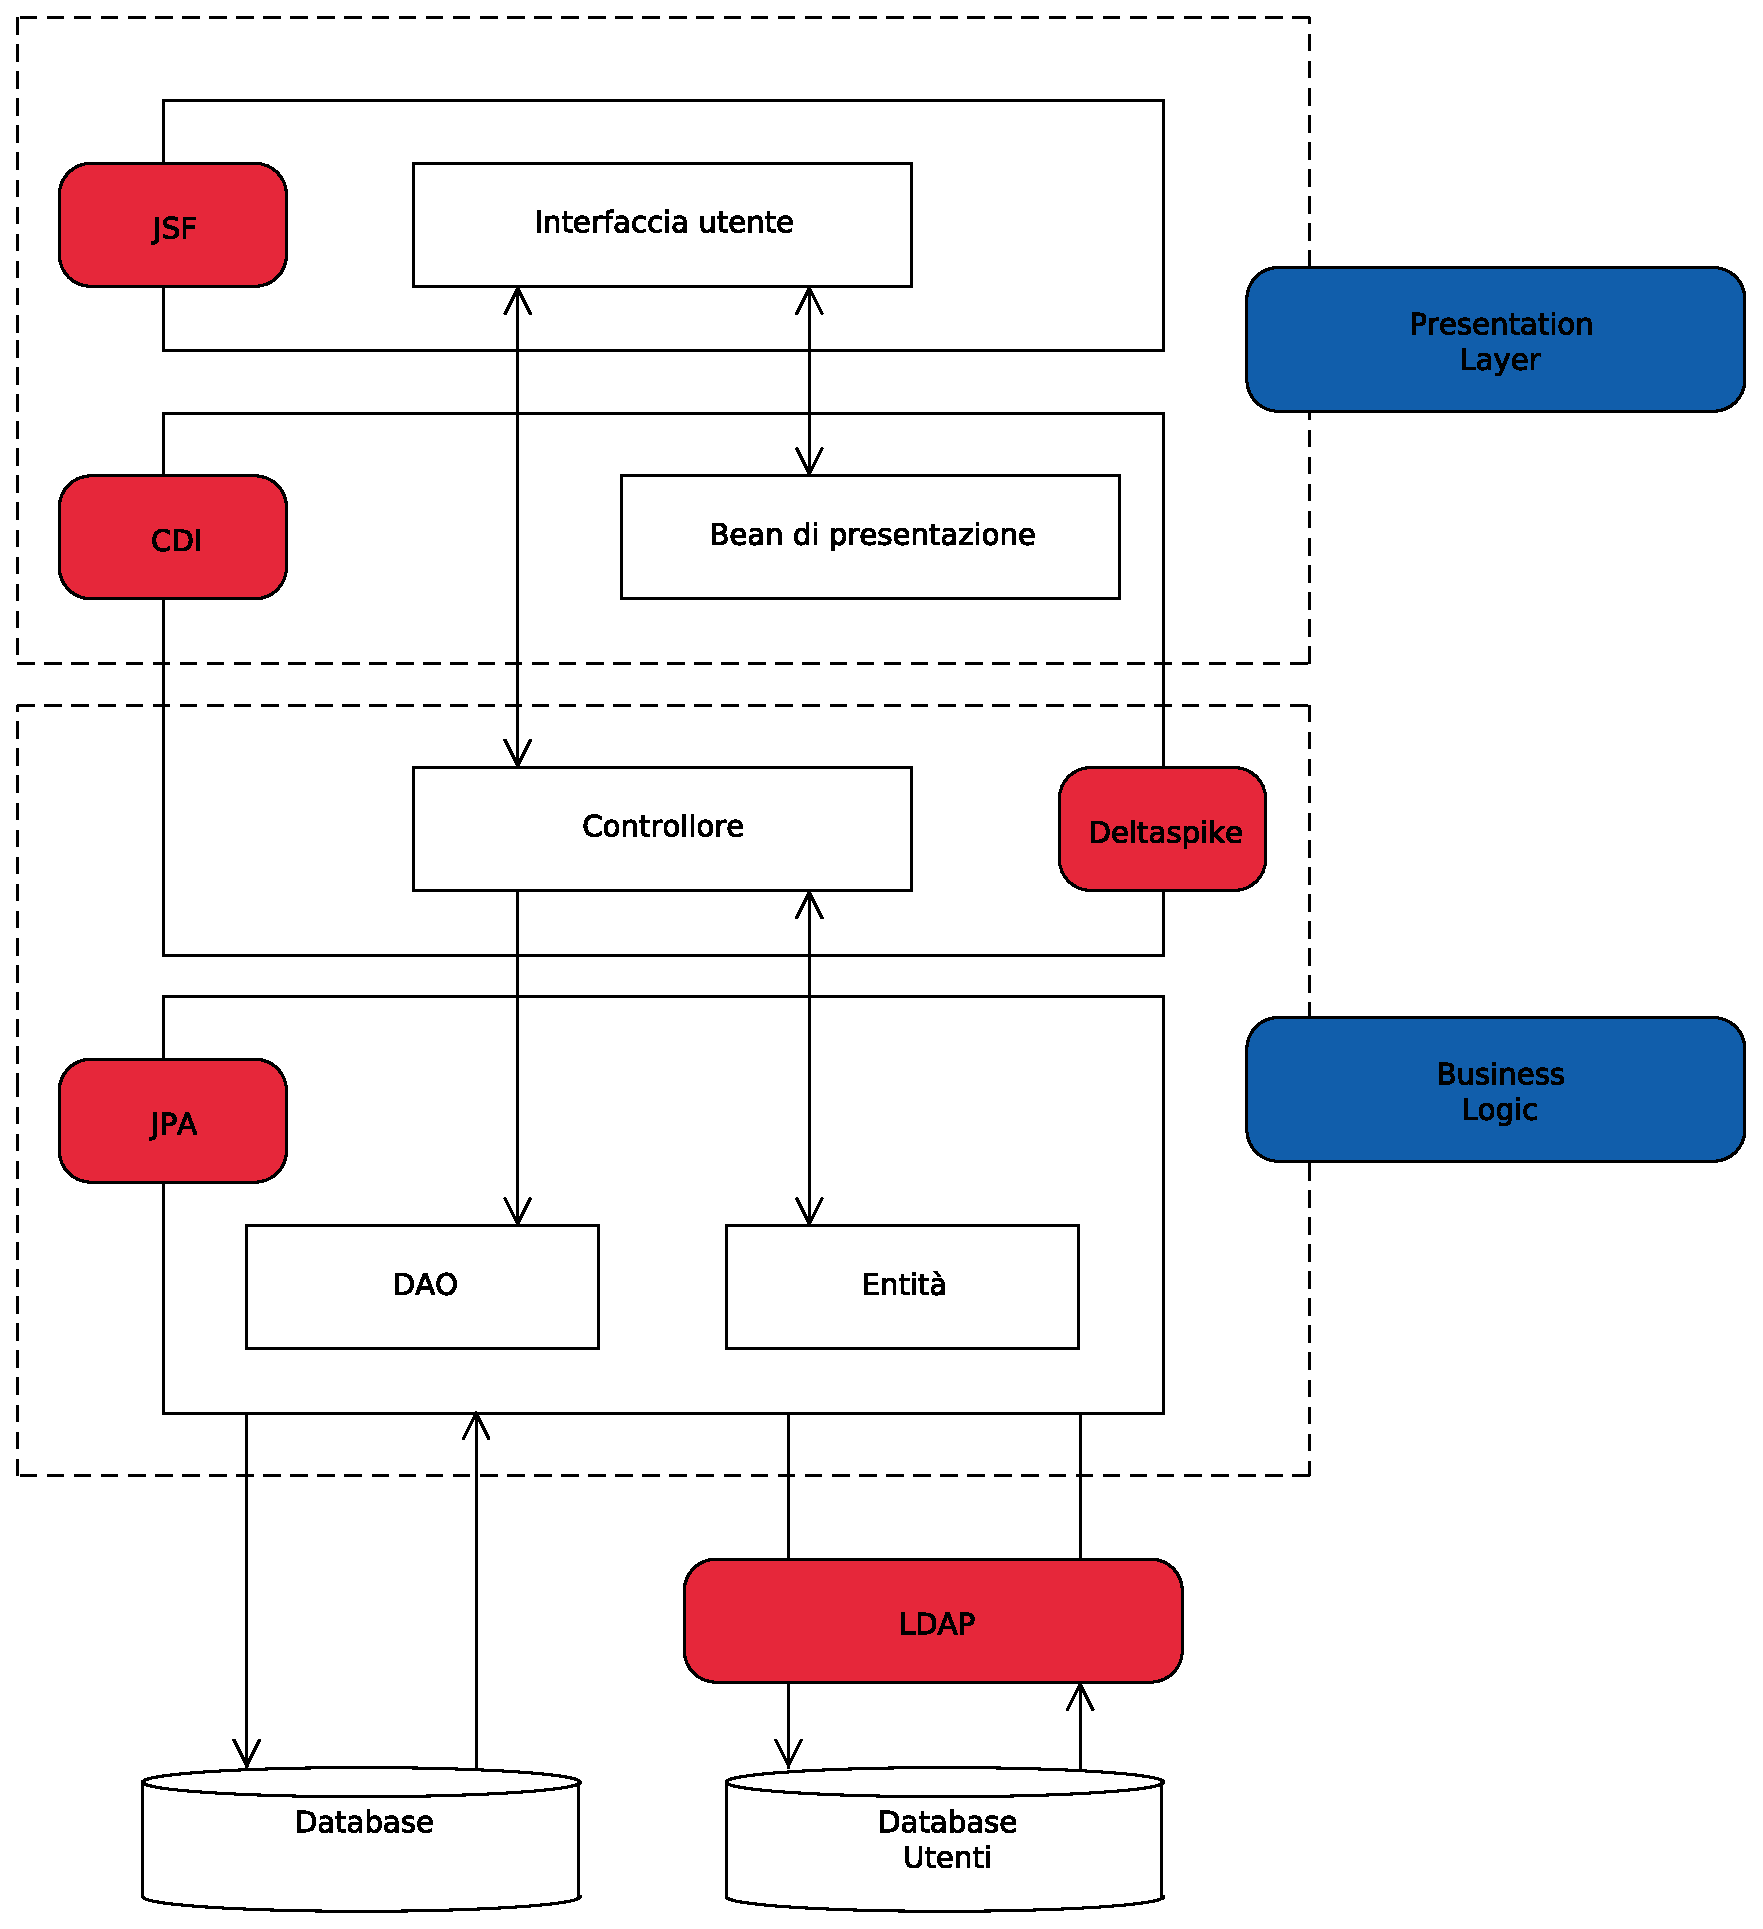
\includegraphics[width=1\textwidth]{tech_architecture_final.eps}

\end{column}
\end{columns}

\end{frame}
%\section[Outline]{}
%\frame{\tableofcontents}

%%%%%%%%%%%%%%%%%%%%%%%%%%%%%%%%%%%%%%%%%%%%%%%%%%

%\section*{}
%\frame{\titlepage}
%%%%%%%%%%%%%%%%%%%%%%%%%%%%%%%%%%%%%%%%%%%%%%%%%%

%\frame{\titlepage}

\end{document} 
